\documentclass[12pt,a4paper]{article}

\usepackage[utf8]{inputenc}
\usepackage[T2A]{fontenc}
\usepackage[russian]{babel}
\usepackage{amsmath,amssymb}
\usepackage{graphicx}
\usepackage{booktabs}
\usepackage{multirow}
\usepackage{geometry}
\usepackage{float}
\usepackage{eso-pic}
\graphicspath{{./}}

\geometry{top=2cm,bottom=2cm,left=2.5cm,right=1.5cm}

\title{\textbf{Лабораторная работа 1.4.5}\\
Изучение колебаний струны}

\author{
    Студент \underline{Шеховцов Василий Максимович}\\
    Группа \underline{Б03-601}\\
    Преподаватель \underline{Ивлев Д.А.}
}

\date{
Московский Физико-технический институт\\
(национальный исследовательский университет)\\
11 ноября 2026 г.
}

\begin{document}

\AddToShipoutPictureFG*{
    \AtPageUpperLeft{
        \hspace{1.5cm}
        \raisebox{-1cm}{
            \makebox[0pt][l]{Шеховцов В.М.}
        }
    }
}

\maketitle

\section{Аннотация}

\textbf{Цель работы:} изучить поперечные стоячие волны на тонкой натянутой струне; измерить собственные частоты колебаний струны и проверить условие образования стоячих волн; измерить скорость распространения поперечных волн на струне и исследовать её зависимость от натяжения струны.

\textbf{Оборудование:} закреплённая на станине стальная струна, набор грузов, электромагнитные датчики, звуковой генератор, двухканальный осциллограф, частотомер.

\section{Теоретические сведения}

Основное свойство струны --- гибкость --- является следствием её большой длины по сравнению с поперечными размерами. Струна практически не сопротивляется изгибу, поэтому изгибные напряжения не учитываются. Сила натяжения $T$ должна значительно превосходить вес струны, чтобы она не провисала.

При малых отклонениях от положения равновесия поперечные колебания струны описываются волновым уравнением
\begin{equation}
    \frac{\partial^2 y}{\partial t^2} = u^2\frac{\partial^2 y}{\partial x^2},
    \label{eq:wave}
\end{equation}
где скорость распространения поперечной волны
\begin{equation}
    u = \sqrt{\frac{T}{\rho_l}},
    \label{eq:u}
\end{equation}
$T$ --- сила натяжения струны, $\rho_l$ --- её погонная плотность (масса на единицу длины). Скорость связана с частотой $\nu$ и длиной волны $\lambda$ соотношением $u = \nu\lambda$.

Для струны длиной $L$ с закреплёнными концами решение уравнения~\eqref{eq:wave} имеет вид стоячей волны $y(x,t)=2a\sin kx\,\sin\omega t$. Концы струны должны быть узлами, откуда следует условие образования стоячих волн: на длине струны укладывается целое число полуволн,
\begin{equation}
    n\,\frac{\lambda_n}{2} = L,\qquad n=1,2,3,\ldots
\end{equation}
Поэтому струна может колебаться лишь на собственных частотах
\begin{equation}
    \nu_n = \frac{u}{2L}\,n = \frac{n}{2L}\sqrt{\frac{T}{\rho_l}}.
    \label{eq:nun}
\end{equation}
Число $n$ равно числу пучностей стоячей волны. Спектр собственных частот определяется длиной, натяжением и погонной плотностью струны и не зависит от модуля Юнга материала.

Колебания поддерживаются вынуждающей силой, поэтому для эффективной раскачки частота генератора должна совпадать с одной из собственных частот (резонанс). Реальные колебания никогда не являются чисто стоячими: из-за потерь энергии при отражении на концах к стоячей волне добавляется малая бегущая компонента, которая переносит энергию вдоль струны и приводит к небольшому <<размытию>> узлов. При слишком большой амплитуде нарушается применимость волнового уравнения (появляются нелинейные эффекты), поэтому возбуждение должно быть слабым.

\section{Экспериментальная установка}

Схема установки приведена на рис.~\ref{fig:setup}. Стальная гитарная струна~1 закреплена горизонтально между стойками~2 и~3 на массивной станине~4. К концу струны, перекинутому через блок, прикреплена платформа с грузами~5, создающими натяжение. Электромагнитный датчик~6, подключённый к звуковому генератору~7, возбуждает колебания струны. Частота измеряется частотомером~10. Колебания регистрирует датчик~8, сигнал с которого подаётся на осциллограф~9.

Возбуждающий датчик располагается вблизи неподвижного конца струны (вблизи узла), регистрирующий --- в пучности. Сила, действующая на струну со стороны датчика, пропорциональна $(B_0+B_\sim)^2\approx B_0^2+2B_0B_\sim$, то есть при $B_\sim\ll B_0$ линейно зависит от тока, а её частота совпадает с частотой генератора.

\begin{figure}[H]
    \centering
    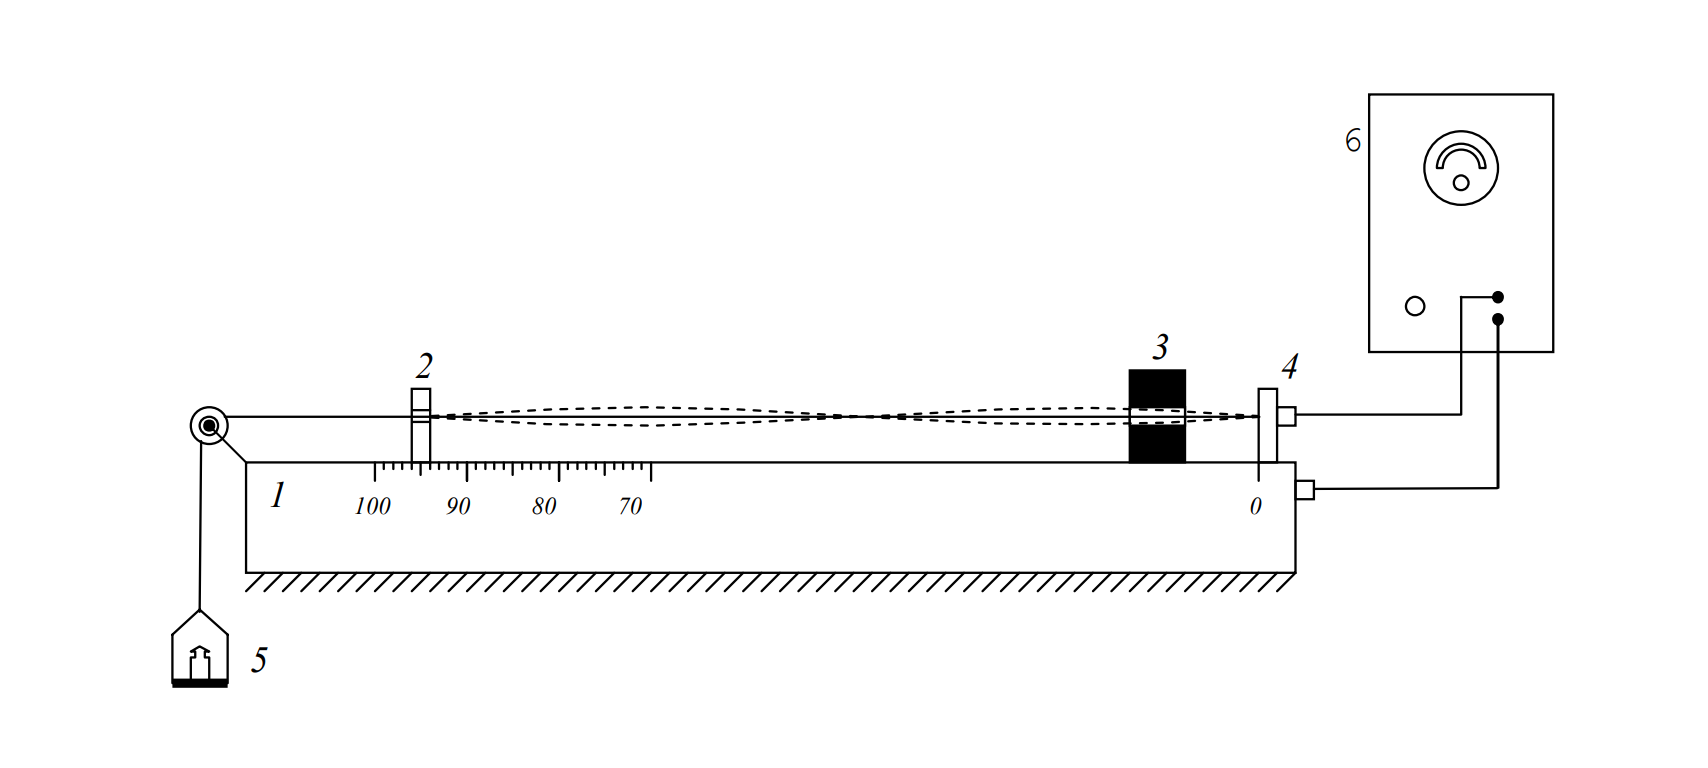
\includegraphics[width=0.85\textwidth]{pic.png}
    \caption{Схема экспериментальной установки}
    \label{fig:setup}
\end{figure}

Длина струны $L = 0{,}500 \pm 0{,}001$~м, табличное значение погонной плотности $\rho_l^{\text{табл}} = 568{,}4$~мг/м $= 5{,}684\cdot10^{-4}$~кг/м.

\section{Обработка результатов}

Резонансные частоты $\nu_n$ измерялись при пяти натяжениях струны. Масса грузов вместе с платформой $m_1=110{,}6+461{,}4+492{,}7=1064{,}7$~г, далее последовательно добавлялись грузы массой $480{,}7$, $500{,}3$, $499{,}1$ и $481{,}7$~г. Сила натяжения $T=mg$, $g=9{,}8$~м/с$^2$. учитывается.

\begin{table}[H]
    \centering
    \caption{Измеренные резонансные частоты $\nu_n$, Гц}
    \begin{tabular}{ccccccccc}
        \toprule
        $m$, г & $T$, Н & $\nu_1$ & $\nu_2$ & $\nu_3$ & $\nu_4$ & $\nu_5$ & $\nu_6$ & $\nu_7$ \\
        \midrule
        1064,7 & 10,434 & 135,3 & 271,6 & 402,1 & 542,2 & 677,0 & 812,9 & 948,9 \\
        1545,4 & 15,145 & 161,4 & 323,2 & 485,9 & 648,4 & 808,3 & 969,6 & 1130,9 \\
        2045,7 & 20,048 & 186,7 & 372,7 & 560,5 & 746,6 & 931,8 & --- & --- \\
        2544,8 & 24,939 & 208,4 & 416,7 & 624,2 & 833,1 & 1041,3 & --- & --- \\
        3026,5 & 29,660 & 230,8 & 455,0 & 682,4 & 909,1 & 1137,1 & --- & --- \\
        \bottomrule
    \end{tabular}
\end{table}

\subsection{Зависимость частоты от номера гармоники}

Согласно~\eqref{eq:nun}, частота линейно зависит от номера гармоники: $\nu_n = k\,n$, где $k=\dfrac{u}{2L}$, и график $\nu_n(n)$ проходит через начало координат (рис.~\ref{fig:nun}).

\begin{figure}[H]
    \centering
    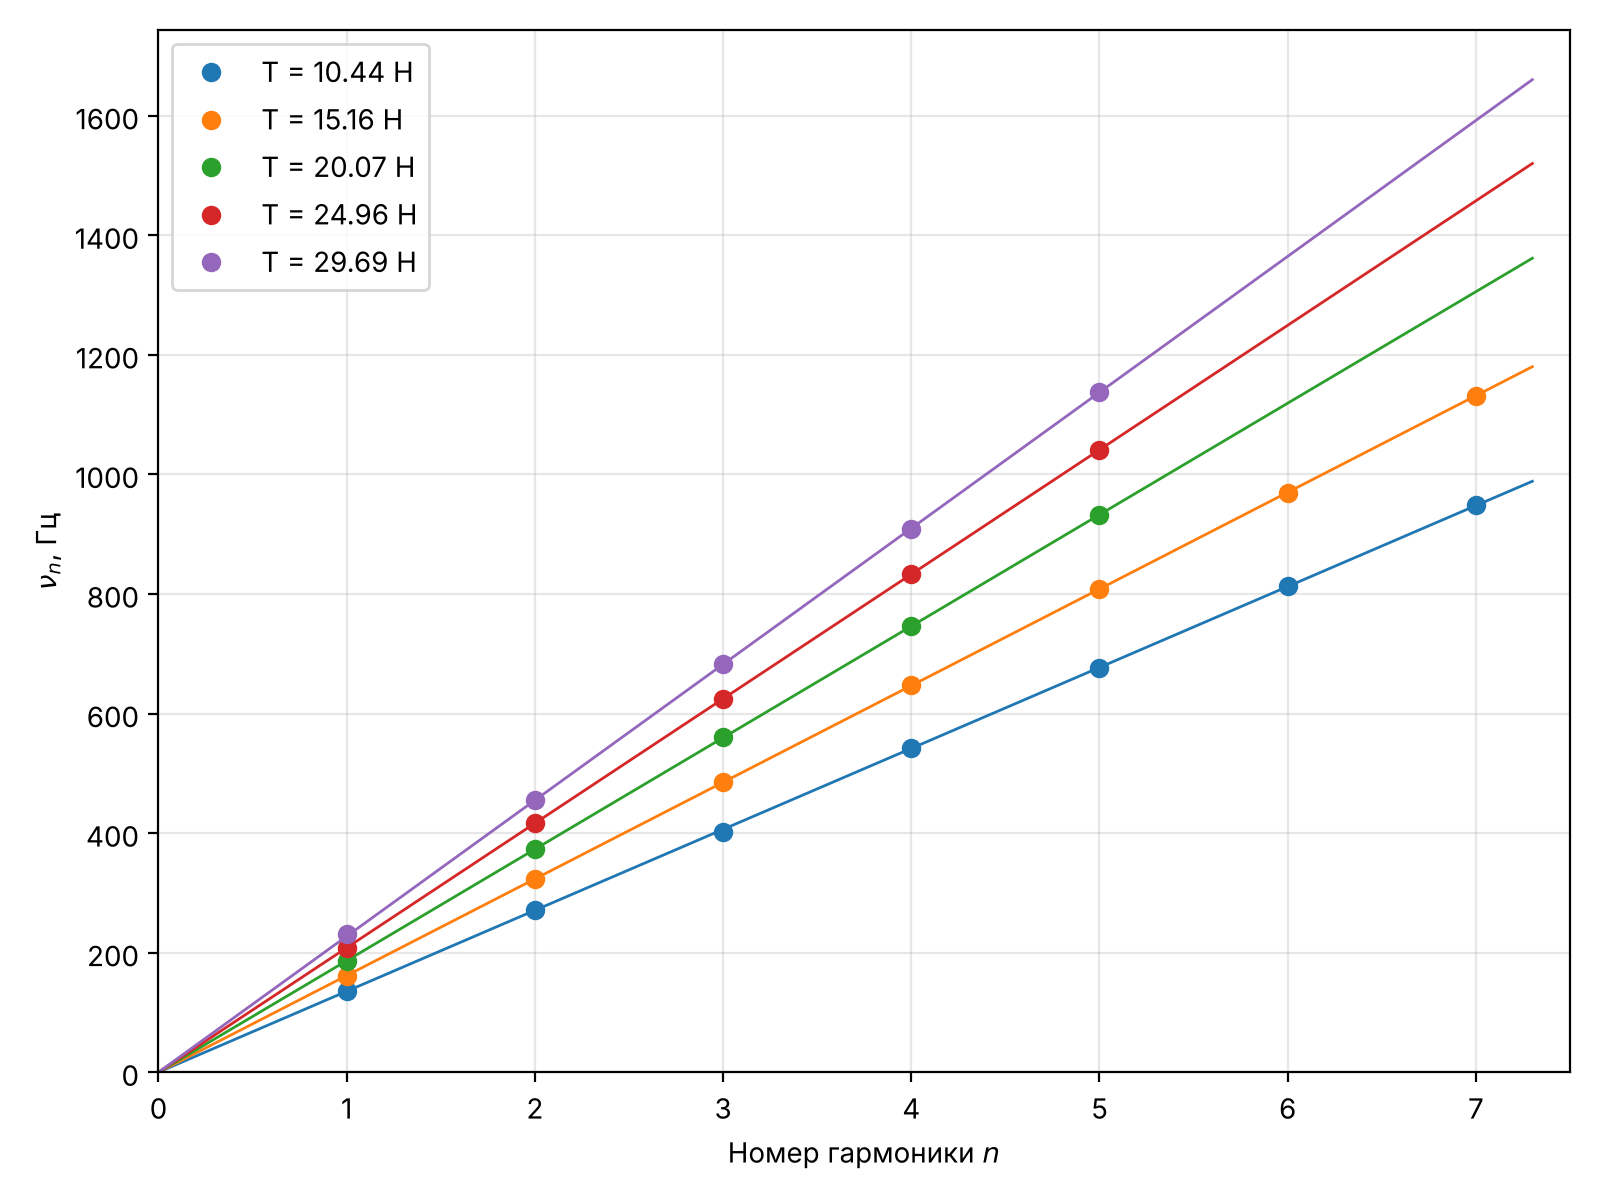
\includegraphics[width=0.85\textwidth]{nu_vs_n.png}
    \caption{Зависимость частоты от номера гармоники для различных натяжений}
    \label{fig:nun}
\end{figure}

Для каждого натяжения коэффициент $k$ находится методом наименьших квадратов для прямой, проходящей через начало координат. Он выбирается так, чтобы сумма $\sum_n(\nu_n-kn)^2$ была минимальной. Приравнивая производную по $k$ нулю, получаем
\begin{equation}
    k=\frac{\langle n\nu_n\rangle}{\langle n^2\rangle}=\frac{\sum n\nu_n}{\sum n^2},
    \qquad
    \sigma_k=\sqrt{\frac{1}{N-1}\left(\frac{\langle \nu_n^2\rangle}{\langle n^2\rangle}-k^2\right)},
    \label{eq:k}
\end{equation}
где $N$ --- число измеренных гармоник. Величина $\sigma_k$ характеризует разброс экспериментальных точек относительно найденной прямой. Скорость волны и её погрешность
\begin{equation}
    u=2Lk,\qquad \sigma_u=2L\sigma_k.
\end{equation}
Погрешность длины струны $\sigma_L$ входит во все $u$ одинаково (это систематическая ошибка), поэтому учитывается один раз при вычислении $\rho_l$.

\textit{Пример расчёта для $T=10{,}434$~Н} ($N=7$):
\begin{equation*}
    \sum n\nu_n = 1\cdot135{,}3+2\cdot271{,}6+3\cdot402{,}1+4\cdot542{,}2+5\cdot677{,}0+6\cdot812{,}9+7\cdot948{,}9 = 18958{,}3,
\end{equation*}
\begin{equation*}
    \sum n^2 = 1+4+9+16+25+36+49=140,\qquad k=\frac{18958{,}3}{140}=135{,}42~\text{Гц},
\end{equation*}
\begin{equation*}
    \sigma_k=\sqrt{\frac{1}{6}\left(\frac{2567284{,}5}{140}-135{,}42^2\right)}
    =\sqrt{\frac{18337{,}75-18337{,}61}{6}}=0{,}15~\text{Гц},
\end{equation*}
\begin{equation*}
    u=2\cdot0{,}500\cdot135{,}42=135{,}4~\text{м/с},\qquad \sigma_u=2\cdot0{,}500\cdot0{,}15=0{,}15~\text{м/с}.
\end{equation*}
Для остальных натяжений расчёт аналогичен, результаты приведены в таблице~\ref{tab:u}.

\begin{table}[H]
    \centering
    \caption{Скорости волн и их сравнение с теорией $u_{\text{теор}}=\sqrt{T/\rho_l^{\text{табл}}}$}
    \label{tab:u}
    \begin{tabular}{ccccc}
        \toprule
        $T$, Н & $k\pm\sigma_k$, Гц & $u_{\text{эксп}}\pm\sigma_u$, м/с & $u_{\text{теор}}$, м/с & отклонение, \% \\
        \midrule
        10,434 & $135{,}42\pm0{,}15$ & $135{,}42\pm0{,}15$ & 135,49 & $-0{,}05$ \\
        15,145 & $161{,}68\pm0{,}07$ & $161{,}68\pm0{,}07$ & 163,23 & $-0{,}95$ \\
        20,048 & $186{,}53\pm0{,}09$ & $186{,}53\pm0{,}09$ & 187,80 & $-0{,}68$ \\
        24,939 & $208{,}24\pm0{,}04$ & $208{,}24\pm0{,}04$ & 209,47 & $-0{,}58$ \\
        29,660 & $227{,}45\pm0{,}23$ & $227{,}45\pm0{,}23$ & 228,43 & $-0{,}43$ \\
        \bottomrule
    \end{tabular}
\end{table}

\subsection{Зависимость скорости от натяжения}

Из~\eqref{eq:u} следует $u^2=T/\rho_l$, то есть график $u^2(T)$ --- прямая, проходящая через начало координат, с наклоном $K=1/\rho_l$ (рис.~\ref{fig:u2T}).

\begin{figure}[H]
    \centering
    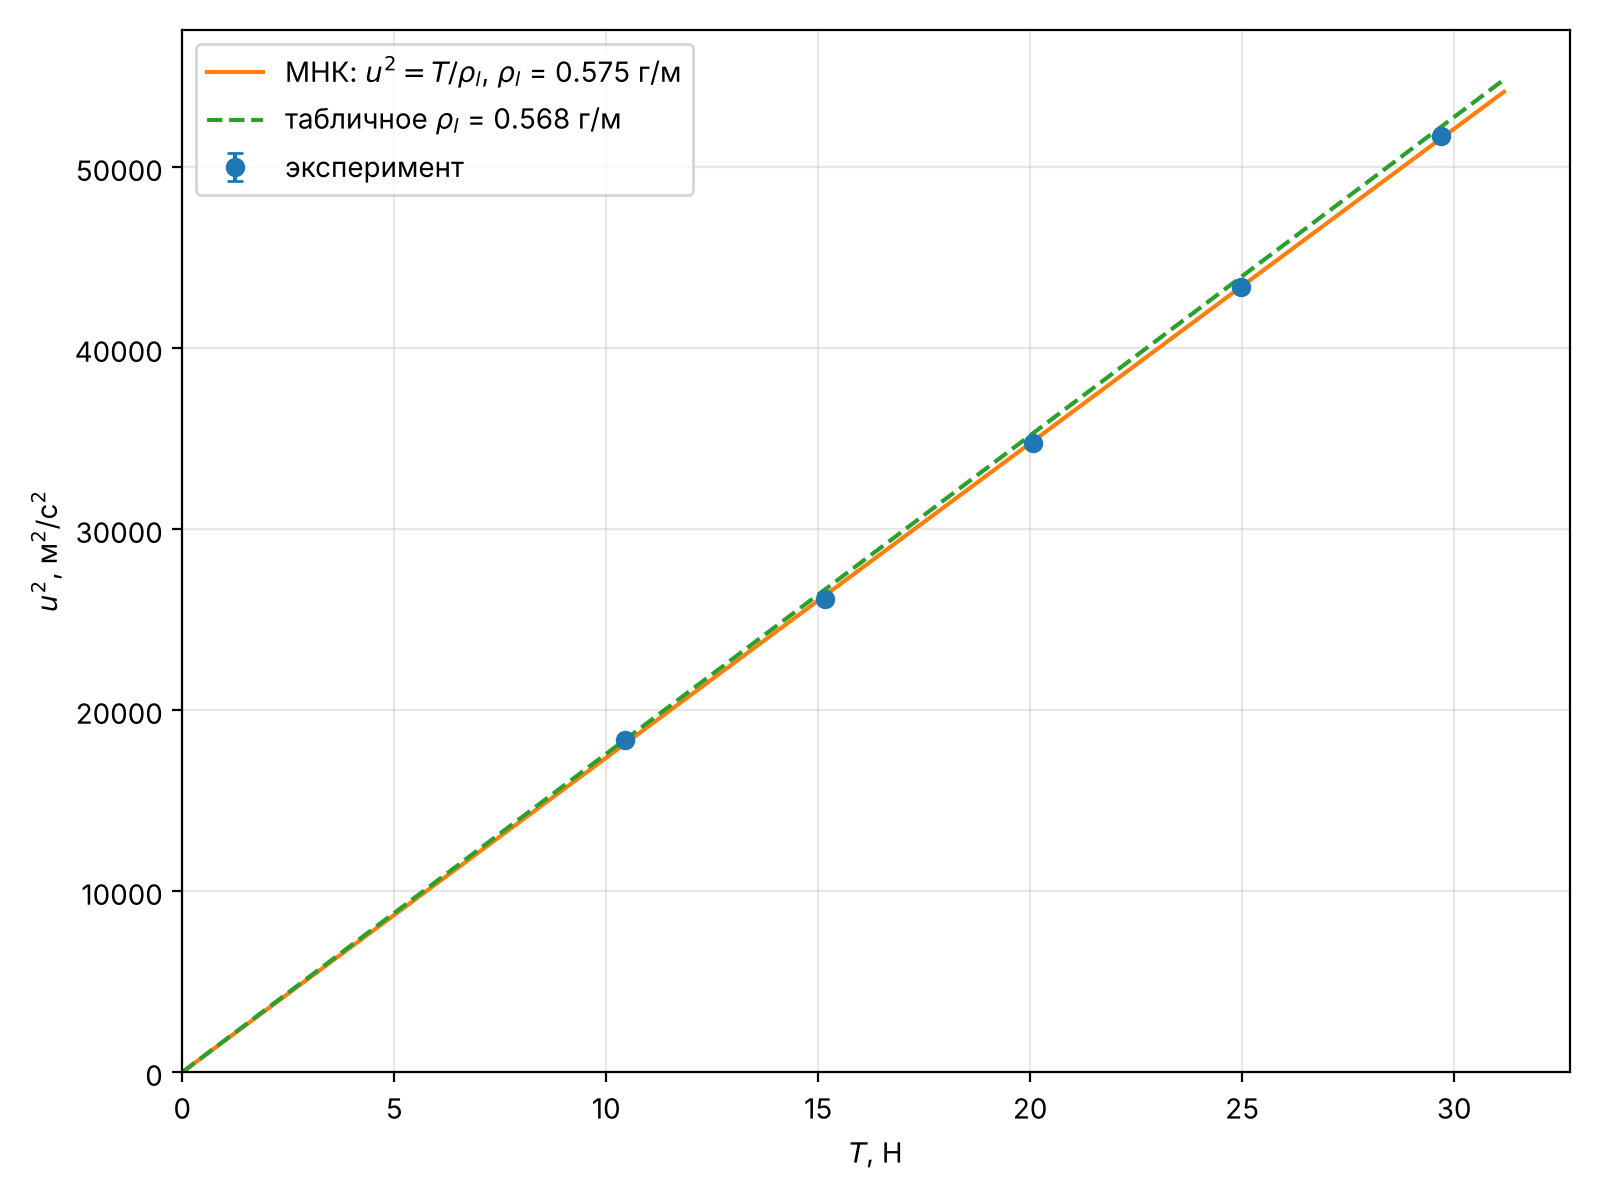
\includegraphics[width=0.85\textwidth]{u2_vs_T.png}
    \caption{Зависимость квадрата скорости от силы натяжения}
    \label{fig:u2T}
\end{figure}

Аналогично предыдущему пункту, методом наименьших квадратов для прямой через начало координат ($N=5$ точек):
\begin{equation}
    K=\frac{\langle Tu^2\rangle}{\langle T^2\rangle}=\frac{\sum T_iu_i^2}{\sum T_i^2},
    \qquad
    \sigma_K=\sqrt{\frac{1}{N-1}\left(\frac{\langle u^4\rangle}{\langle T^2\rangle}-K^2\right)}.
\end{equation}
Подстановка: $\sum T_iu_i^2=3\,900\,629$~Н$\cdot$м$^2$/с$^2$, $\sum T_i^2=2241{,}81$~Н$^2$, $\sum u_i^4=6{,}787\cdot10^{9}$~м$^4$/с$^4$,
\begin{equation*}
    K=\frac{3\,900\,629}{2241{,}81}=1739{,}9~\text{м/кг},
\end{equation*}
\begin{equation*}
    \sigma_K=\sqrt{\frac{1}{4}\left(\frac{6{,}787\cdot10^{9}}{2241{,}81}-1739{,}9^2\right)}
    =\sqrt{\frac{3\,027\,464-3\,027\,418}{4}}=3{,}4~\text{м/кг}.
\end{equation*}
Погонная плотность и её погрешность:
\begin{equation*}
    \rho_l=\frac{1}{K}=\frac{1}{1739{,}9}=574{,}7\cdot10^{-6}~\text{кг/м},\qquad
    \sigma_{\rho}^{\text{случ}}=\rho_l\frac{\sigma_K}{K}=574{,}7\cdot\frac{3{,}4}{1739{,}9}=1{,}1\cdot10^{-6}~\text{кг/м}.
\end{equation*}
Так как $u\propto L$, а $\rho_l=T/u^2\propto L^{-2}$, погрешность длины даёт вклад
\begin{equation*}
    \sigma_{\rho}^{L}=\rho_l\cdot\frac{2\sigma_L}{L}=574{,}7\cdot\frac{2\cdot0{,}001}{0{,}500}=2{,}3\cdot10^{-6}~\text{кг/м}.
\end{equation*}
Полная погрешность $\sigma_\rho=\sqrt{(\sigma_\rho^{\text{случ}})^2+(\sigma_\rho^{L})^2}=2{,}6\cdot10^{-6}$~кг/м. Окончательный результат:
\begin{equation}
    \rho_l^{\text{эксп}} = (574{,}7\pm2{,}6)\cdot10^{-6}\ \text{кг/м}.
\end{equation}

Для контроля $\rho_l$ можно вычислить для каждого натяжения отдельно: $\rho_i=T_i/u_i^2$ даёт $569{,}0$; $579{,}4$; $576{,}2$; $575{,}1$; $573{,}3$~мг/м. Все значения лежат в пределах 1\% от среднего, что согласуется с результатом МНК.

\section{Обсуждение результатов}

Полученное значение $\rho_l^{\text{эксп}}=(574{,}7\pm2{,}6)$~мг/м отличается от табличного $\rho_l^{\text{табл}}=568{,}4$~мг/м на $1{,}1\%$, то есть на $2{,}5\sigma_\rho$. Скорости, измеренные при четырёх натяжениях из пяти, оказываются на $0{,}4$--$1{,}0\%$ ниже теоретических, что и приводит к завышению $\rho_l$. Знак отклонения у них одинаков, поэтому оно является скорее систематическим, чем случайным.

Возможные причины: трение в блоке, из-за которого реальное натяжение струны меньше $mg$; влияние зажима струны в стойке~3, который при затяжке может изменять натяжение и эффективную длину колеблющегося участка.

\section{Вывод}

В ходе работы были изучены стоячие волны на струне. Экспериментально подтверждено условие образования стоячих волн: частота резонанса пропорциональна номеру гармоники ($\nu_n\propto n$, графики --- прямые через начало координат). Проверена зависимость скорости поперечных волн от натяжения ($u^2\propto T$). Экспериментально определена погонная плотность струны $\rho_l=(574{,}7\pm2{,}6)$~мг/м, которая отличается от табличного значения $568{,}4$~мг/м на $1{,}1\%$.

\end{document}